\subsection{How is the concept of monitoring implemented in Ambari and Chukwa?}
\label{subsec:Implementation}
After defining monitoring and its Use Cases, two Software Solutions for monitoring in an \hadoop environment are introduced.

\subsubsection{Ambari}
\amb is ``the only 100\% open source framework''~\cite{Sako2013} that allows the user to monitor, manage and install Hadoop.\cite{ApacheSoftwareFoundation2015} It has the ability to start, stop and configure Hadoop processes automatically on clusters, without any intervention of the user.\cite{Hortonworks2013} \amb was developed to simplify the use of Hadoop.\cite{Hortonworks2013}

\amb architecture can be divided in components. First the \amb Web which is the main platform for users to log in and give up request that should be run through Ambari.~\cite{Sako} It builds the main interface for any interactions between user and application.\cite{Sako} Through \amb Web all the monitoring processes are visualized. 

Secondly, the \amb Server consists of several components.\cite{Sako} The (REST-) API is connected to different web applications, the most important one is \amb Web.\cite{Sako} Other interfaces, like Microsoft System Centre, are applications that allow the user to analyse or integrate data and conclusions to other programs of the user.\cite{Hortonworks2013} The results of the analysis is accessible through \amb Web on the monitoring screens.\cite{Sako}

The connection between \amb and \hadoop is done by the \amb Agents.\cite{Sako} During setup, \amb Server will install the \amb Agent Software on each host. The Agent will sent a regular heartbeat to the server for communication. The server answers with an instruction for the Agent or sends a confirmation about his current life-status.\cite{Sako} All hosts are connected to the clusters by \hadoop.\cite{Sako}

\begin{figure}
  \centering
  % https://docs.google.com/open?id=1A3TbXPEQeknqWxxX811XHG7pcQOuMEFDmo_hl8LlfYk
  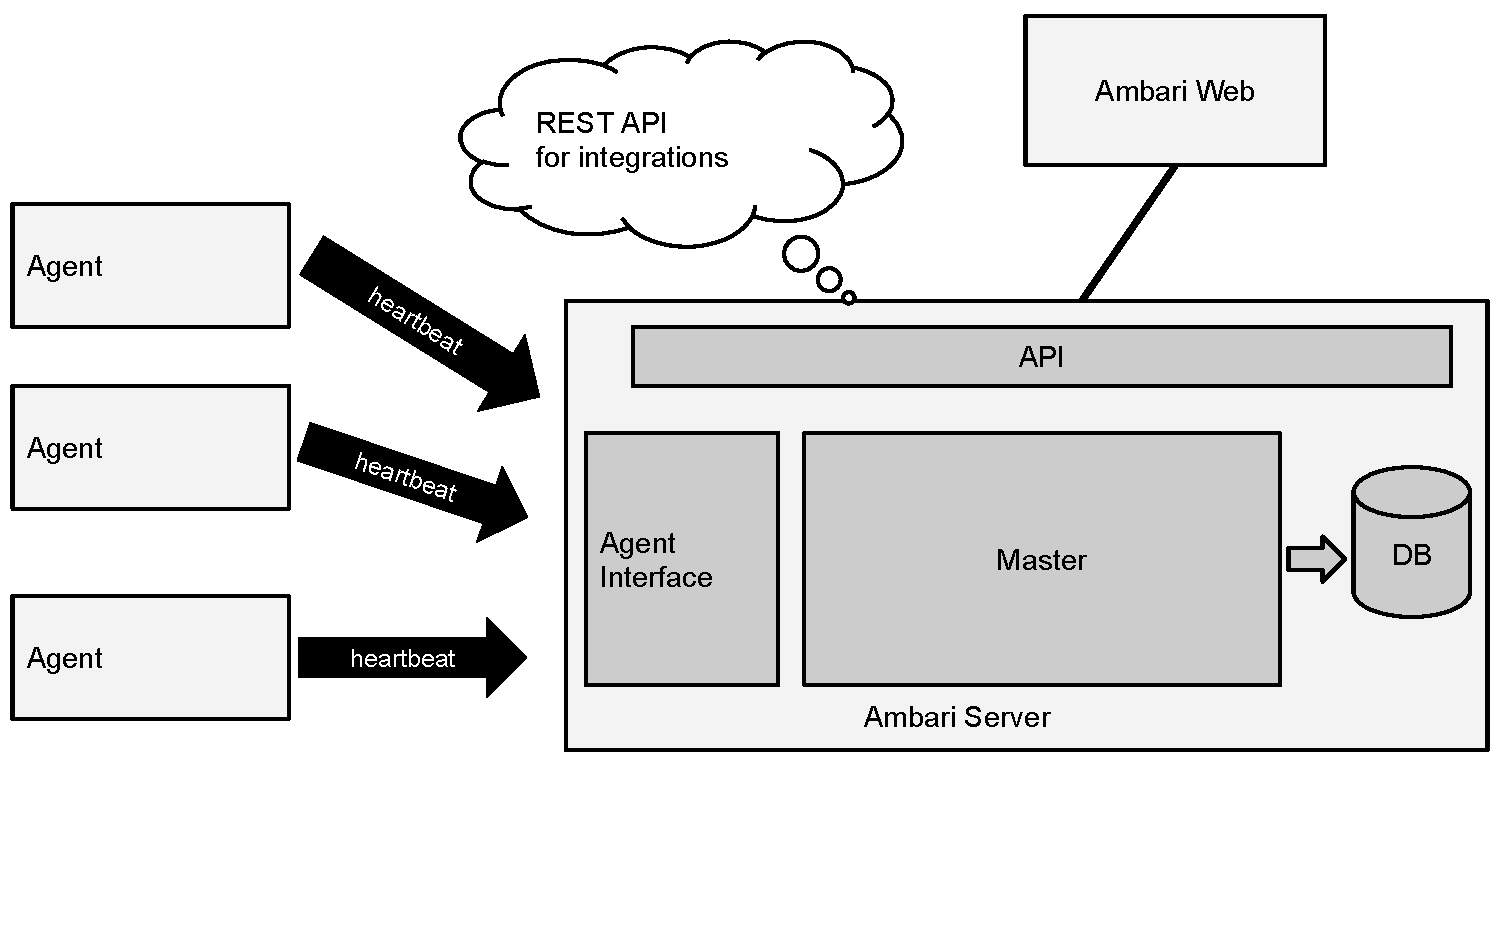
\includegraphics[width=\linewidth,clip=true,trim=0 3cm 0 0]{images/AmbariArchitecture}
  \caption{Ambaris Architecture~\cite{Sako, Sako2013}}
  \label{fig:AmbariArchitecture}
\end{figure}

The concept of monitoring is given in two specific ways with \amb. 
It has knowledge about every nodes health and its data.~\cite{Foley2012} 
It can provide and improve the health situation of a Hadoop cluster and analyse the data in ways there are useful for the user.~\cite{Foley2012} 
The user has an overview on the current situation through the Web application.~\cite{Foley2012} 
\amb divides the monitoring process in three parts.~\cite{Foley2012} 
The first one is the list of all the applications \amb is running on each connected cluster. 
It shows the name, status and number of clusters that are ok, and the ones that need to get fixed.~\cite{Foley2012} 
The second part is explaining all the technical details about the application, such as storing space and running time.~\cite{Foley2012} 
The last part is aimed to show illustratively how long and effective an application has been running on a node.~\cite{Foley2012} 
Based on this data the user can give up requests to change the applications or add more clusters into one process, through the API.~\cite{Sako} 
\amb then will install a new application automatically to the cluster. This command is sent as a response to a heartbeat signal from an \amb Agent. \cite{Sako} 
\amb has the ability of installing and giving a breve overlook about the health of the system; its not capable of analysing the data qualitatively.\cite{Sako}


\subsubsection{Chukwa}
\chuklong is ``a data collection system for monitoring and analyzing large distributed systems.''~\cite{Boulona}
It is built to support log handling on scalable Hadoop clusters. 
Further, it allows ``[c]ross system analysis''~\cite{ChukwaPoster} 
\chuk is developed at Yahoo! and ``is built on top of HDFS and Map-Reduce.''~\cite{Rabkin2008a}
Its main non-functional goals are low footprint on System Usage (less than 5\%) and minimal changes to user workflow.~\cite{Rabkin2010}
``All (..) data [is] in one place''~\cite{ChukwaPoster} eventually.

\paragraph{The process}
For processing Log files and Application Metrics, \chuk starts on the producing machine, which is running a \chuk Agent. 
This piece of Java Software is constantly gathering Application Logs and Metrics from pre-configured locations. 
This can be \textit{syslog} as well as an Application specific location. 
Each Source is fetched by a so called \textit{Adaptor}.~\cite{ChukwaAdminAgent}

\begin{figure}
  \centering
  % https://docs.google.com/open?id=11xCUWZ94zbUa4eqhoScjMmfIL2pI-IkDx02qvcCXohY
  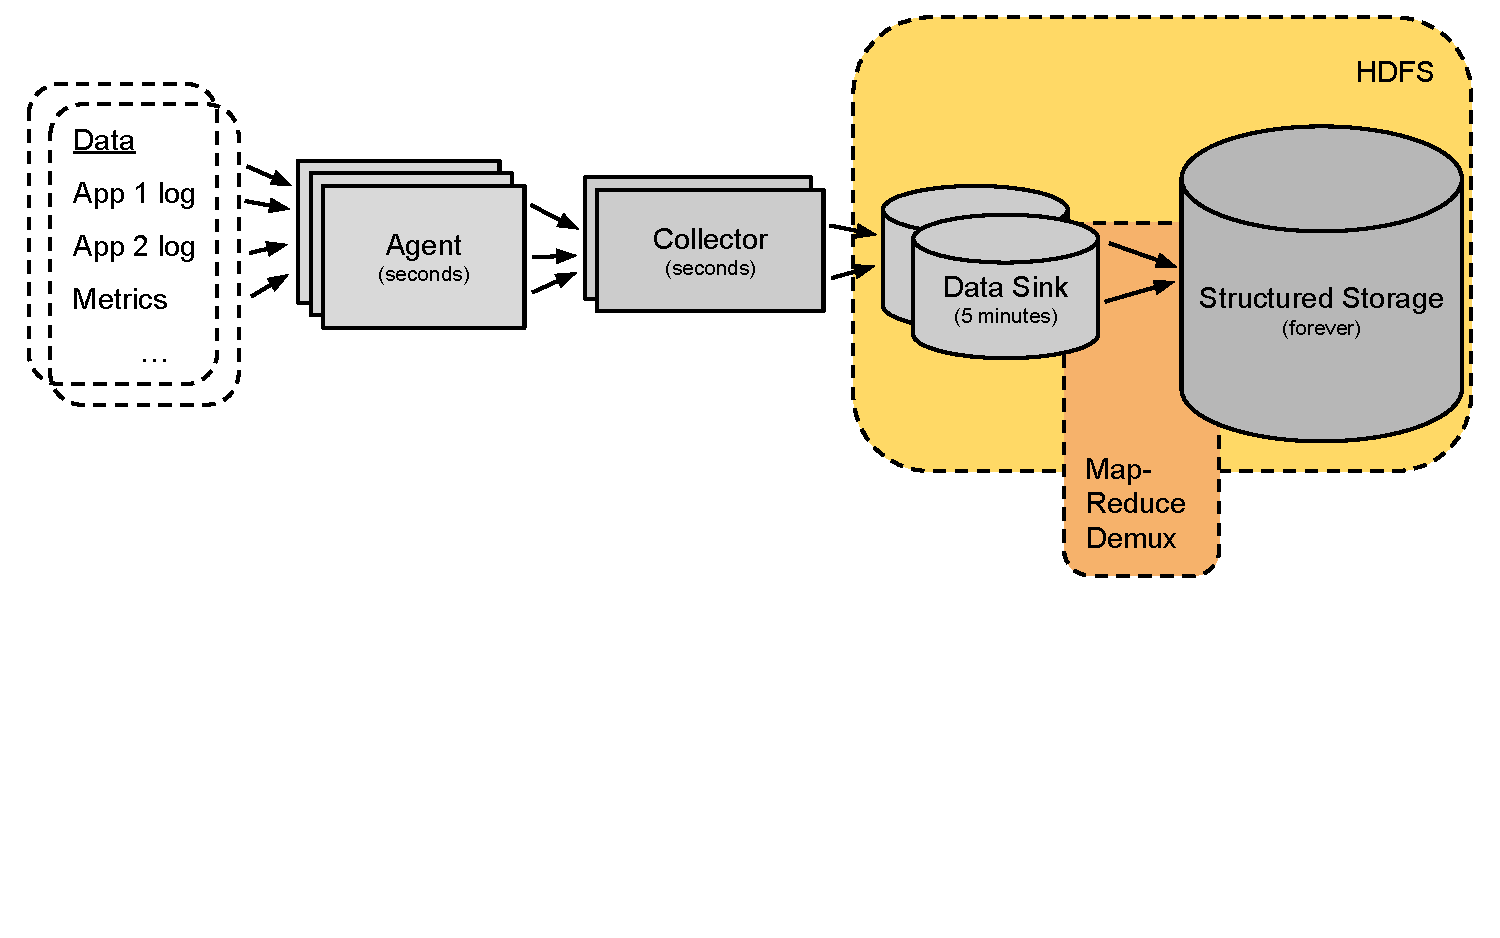
\includegraphics[width=\linewidth,clip=true,trim=0 6cm 0 0]{images/ChukwaArchitecture}
  \caption{Chukwas Architecture~\cite{Rabkin2008}}
  \label{fig:ChukwaArchitecture}
\end{figure}

The Agent is then pushing the data to a so called \textit{Collector}, as described on Figure~\ref{fig:ChukwaArchitecture}.
This is another piece of Java Software, running on a dedicated \chuk instance. 
The \textit{Collector}s job is collecting data from multiple Nodes in the Cluster, as well as archiving and post-processing the data.~\cite{Jose2014}
First, the collected information is stored in \textit{Data Sink} Files. 
Here, data from multiple Nodes gets written in the same file, which can be seen as a Queue for processing.
Every few minutes, the \textit{Data Sink} File is closed. (Files cannot be processed, while data is written to them.)
All available \textit{Data Sink} files will be processed by a pair of Demux \mr jobs.~\cite{Boulona} 


As described by Boulon et al., the \mr processing should produce insights about 
``needs for accounting, capacity planning, performance characterization, utilization'', 
``reduc[e] the number and extent of outages'', 
``reduc[e] the number of false alerts and increasing the value and confidence level of true alerts'' and 
``reduc[e] the time and effort required to identify and resolve cluster issues.''~\cite{Boulonb}

To achieve these goals, ``the first job simply archives all the collected data, without processing or interpreting it. 
The second job parses out structured data from some of the logs, and loads this structured data into a data store.''~\cite{Boulona} 

% reduce can be customised. https://chukwa.apache.org/docs/r0.4.0/programming.html

\paragraph{The Storage}
\label{par:chukStoreage}
The \mr jobs will \demux data out of the \textit{sink} files and into structured storage.~\cite{Boulonb} 
\chuk supports multiple, pluggable storage formats, which ``also aids integration with legacy systems. Chukwa also offers the flexibility to support other data sources, such as syslog or local IPC.''~\cite{Rabkin2010a} 

Currently, \chuk uses \hdfs files, ``one file per cluster, per data type, and time period. (..) [Which is only an] interim solution''~\cite{Boulona} 
The development team is evaluating different data-stores, which are more suitable for the purpose and allow structured querying, also.
Possible storage systems for the future include Hive, HBase or Hypertable. Also local installations of relational Databases might be an option.~\cite{Boulonb} Last option depends on the amount of data stored.

\textit{Hive} is potentially a good fit. It is still based on \hdfs files, but adds a new layer of organisational functionality like ``Organization into Tables'' or a ``SQL like query language over object data stored in Tables.''~\cite{Sarma08}